\section{Observing Performance}
\label{sec:performance}

\subsection{Realized footprint and cadence}
\label{sec:coverage}

The 39,590 validated exposures correspond to 329.95~hr of open-shutter
time. This is the sum of exposure durations, excluding readout,
slews, and other overheads. Table~\ref{tab:results} collects the principal
performance measurements and identifies their statistical samples.

We derive each footprint from the corners of its verified L2 image
WCS, including the archived TPV distortion solution. Overlaps are
combined on a HEALPix grid \citep{Gorski2005}, using a pixel-center
test for membership in each footprint polygon. The area covered at
least once is $10,928.1~\degsq$. A second measure first counts visits
within each physical observing night and then takes the union of
sky pixels receiving at least three exposures on any one night;
this area is $10,470.6~\degsq$. The adopted totals use $N_{\rm side}=1024$ and measure the geometric
footprint of the validated exposures.

Figure~\ref{fig:coverage} compares the accumulated exposure coverage
with the spatial distribution of the known-object associations.
Both show the ecliptic observing region, but the quantities have
different weightings. Exposure density measures where the camera
observed, whereas association density also depends on the population,
geometry, sensitivity, and catalog selection. The footprint uses the actual WCS pointings.

\begin{figure}[tbp]
\centering
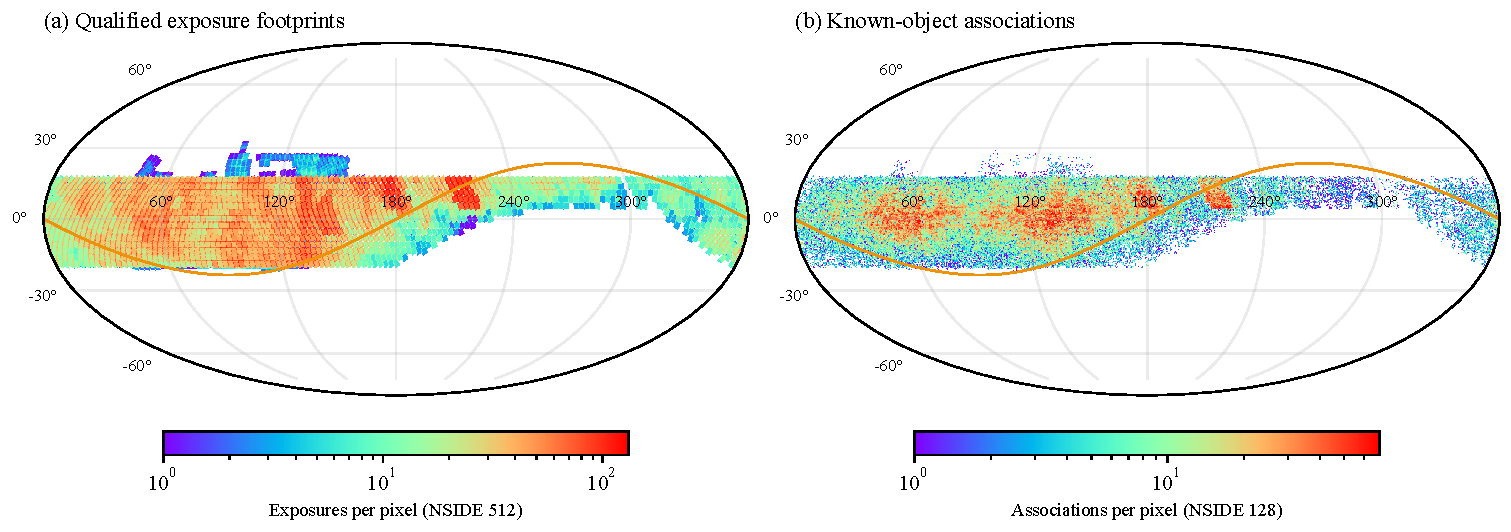
\includegraphics[width=\linewidth]{fig03_coverage_and_known_sky.pdf}
\caption{The accumulated \SHARP\ observations in J2000 ecliptic
longitude and latitude. (a) Number of validated exposures covering
each HEALPix pixel, using actual image WCS footprints and
$N_{\rm side}=512$. (b) Number of primary $1\asec$ known-object
associations per pixel at $N_{\rm side}=128$. The orange curve is
the celestial equator. The color scales are logarithmic and
represent different statistical units and pixel areas. The
geometric areas quoted in the text are evaluated at
$N_{\rm side}=1024$.}
\label{fig:coverage}
\end{figure}

To measure the within-night cadence, we group exposures by physical
observing night, recorded field identifier, and actual WCS pointing.
Complete-link grouping requires any two centers in a group to be
separated by at most $0.30^\circ$, approximately one tenth of the
camera width, so that images with substantially different pointings
are assigned to separate observing sequences.

The resulting 14,400 field--night pointing groups contain 2,651
single visits, 2,039 pairs, and 9,710 sequences with at least three
visits. Thus 67.43\% of groups supply three or more validated
exposures. The median interval among the 25,190 adjacent
exposure pairs is 37.65~min, with a 16th--84th percentile range of
28.37--41.92~min. For the groups with at least three visits, the
median first-to-last span is 78.23~min, with a corresponding range
of 61.93--91.50~min.

Figure~\ref{fig:cadence} shows the observing activity and cadence
distributions. The observed spacing is longer than the nominal
30~min design value, and the distributions include incomplete and
extended sequences. The cumulative area that has ever received
three within-night exposures and the fraction of individual
field--night groups completing three visits answer different
questions; both are needed to describe the sampling available
for moving-source searches.

\begin{figure}[tbp]
\centering
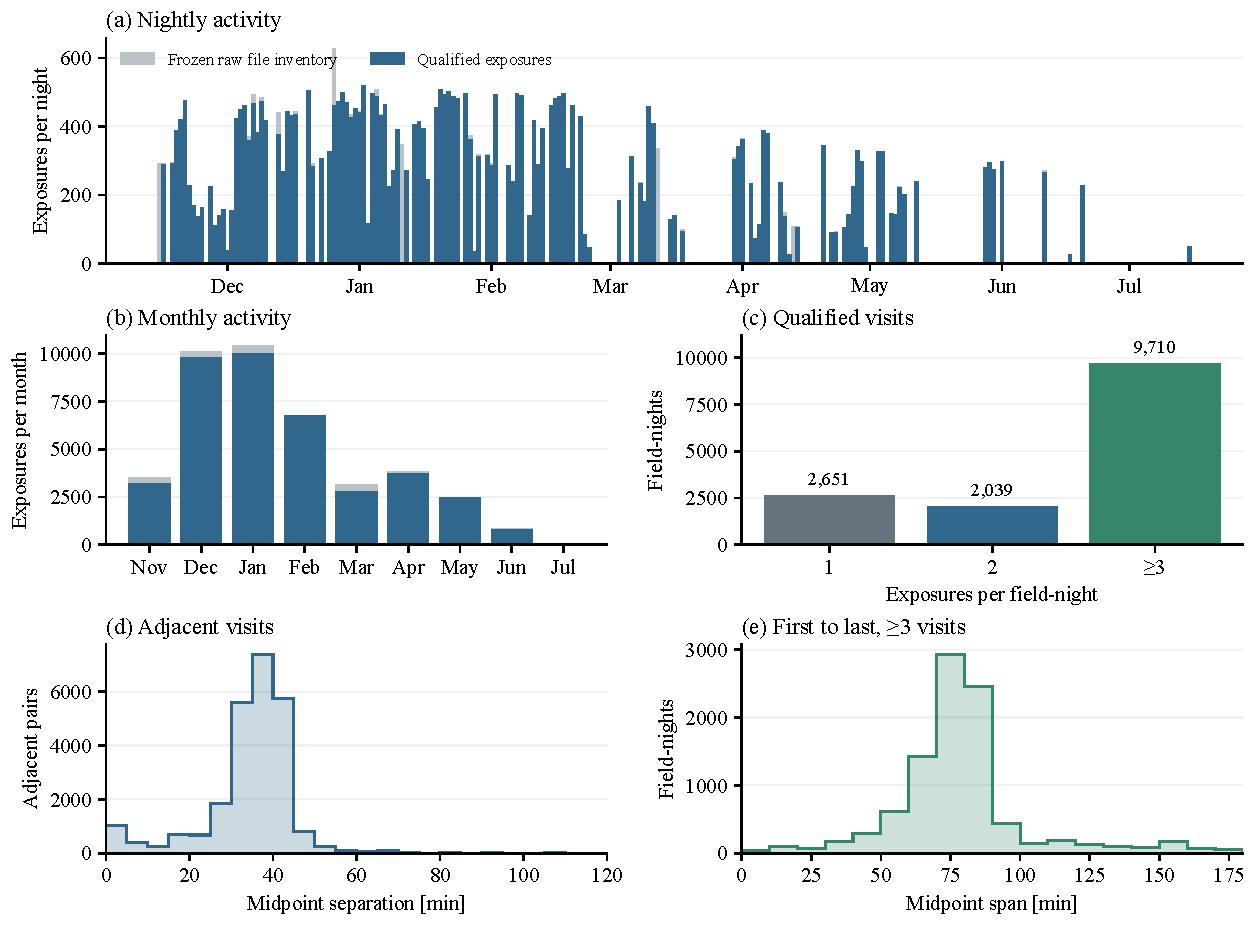
\includegraphics[width=0.96\linewidth]{fig04_activity_and_cadence.pdf}
\caption{Observing activity and realized cadence. (a,b) Nightly
and monthly counts in the original raw-file inventory and the
validated exposure sample. Both counts in (a,b) are grouped by
archive-directory date for a direct inventory comparison.
Panels (c--e) use exposure midpoints and local-noon observing
nights. (c) Number of validated visits in each of the
14,400 field--night pointing groups. (d) Midpoint separation of
25,190 adjacent exposure pairs within those groups. (e)
First-to-last midpoint span for the 9,710 groups containing at
least three visits. The plotted interval ranges emphasize the
main distributions; the accompanying machine-readable histograms
retain the full tails.}
\label{fig:cadence}
\end{figure}

\begin{table}[tbp]
\centering
\caption{Principal Measurements of the Initial Campaign}
\label{tab:results}
\begin{tabular}{ll}
\toprule
Quantity & Measured value\\
\midrule
\multicolumn{2}{l}{\textit{Validated exposure sample}}\\
Exposures / physical observing nights & 39,590 / 129\\
Open-shutter time & 329.95~hr\\
Geometric area with at least one exposure & $10,928.1~\degsq$\\
Area ever reaching three exposures in one night & $10,470.6~\degsq$\\
Field--night groups with at least three visits & 9,710 / 14,400 (67.43\%)\\
Median adjacent-visit interval & 37.65~min\\
Median span of sequences with at least three visits & 78.23~min\\
Median catalog $5\sigma$ model depth & 20.25~mag\\
Model-depth interquartile range & 19.76--20.58~mag\\
\midrule
\multicolumn{2}{l}{\textit{Primary $1\asec$ associations in validated exposures}}\\
Associations / catalog identities & 531,612 / 58,281\\
Identities in the main-belt orbital region & 55,791 (95.73\%)\\
Median radial O$-$C separation & $0.263\asec$\\
Robust scatter in $\Delta\alpha\cos\delta$ / $\Delta\delta$ & $0.222\asec$ / $0.215\asec$\\
\midrule
\multicolumn{2}{l}{\textit{Linkage assessment and reviewed candidates}}\\
Historical conditional retention & 75,899 / 102,347 (74.16\%)\\
After exposure and night validation & 75,467 / 101,784 (74.14\%)\\
Image-reviewed single-night linkages & 58\\
Measurements / nights in retained linkages & 179 / 34\\
\bottomrule
\end{tabular}
\tablecomments{Model depth is defined by Equation~\ref{eq:depth}.
Astrometric scatter is $0.7413\,\mathrm{IQR}$ within the primary
association selection. The two retention rows use the cohorts defined in
Section~\ref{sec:retention_results}. All 179 reviewed candidate
measurements belong to validated exposures.}
\end{table}

\subsection{Photometric and astrometric performance}
\label{sec:photometry}

The validated images have a median catalog image FWHM of
$3.58\asec$, with an interquartile range of
$3.16$--$4.24\asec$. The per-exposure depth summary uses the
archived L2 quantity \texttt{MLIM}. Its calculation is
\begin{align}
F_{5,\rm ADU} &=
\frac{5}{g_{\rm e}}\left[(s_{\rm ADU}g_{\rm e}+r_{\rm e}^{\,2})
                 \,\pi\left(\frac{w_{\rm pix}}{2}\right)^2
                 \right]^{1/2},\\
m_{5,\rm model} &= ZP-2.5\log_{10} F_{5,\rm ADU},
\label{eq:depth}
\end{align}
where $s_{\rm ADU}$ is the sky level per pixel, $g_{\rm e}$ is
the gain in electrons per ADU, $r_{\rm e}$ is the read noise in
electrons, $w_{\rm pix}$ is the image FWHM in pixels, and $ZP$
is the exposure's zero point for the 18-pixel-diameter reference
aperture. This background-plus-read-noise model uses a circular noise
area with radius FWHM/2. It applies no separate encircled-energy
correction at that radius and does not use the eight-pixel aperture
correction in Equation~\ref{eq:apercal}.

The median model depth is 20.25~mag, and the interquartile range
is 19.76--20.58~mag (Figure~\ref{fig:quality}a). Its noise
aperture differs from the fixed eight-pixel-diameter aperture used for
\gaper. We therefore report this value specifically as the catalog
background-noise model depth.

Figure~\ref{fig:quality}b shows the cataloged aperture-magnitude
uncertainties of unflagged known-object associations with positive
aperture fluxes and errors. An independent
short-timescale check uses 18 archived L2 catalogs in six selected
field--night sequences. We match isolated, unflagged, stellar
detections between visits and estimate a per-epoch scatter from
their magnitude differences,
\begin{equation}
\sigma_{\rm epoch} =
\frac{0.7413\,\mathrm{IQR}(\Delta g_{\rm aper})}{\sqrt{2}}.
\label{eq:repeatability}
\end{equation}
This estimator converts the interquartile spread to a
Gaussian-equivalent scatter and attributes comparable noise
to the two epochs.

At $15.5\leq\gaper<16$, the estimated scatter is 0.0118~mag,
compared with a median reported uncertainty of 0.0115~mag.
At $17.5\leq\gaper<18$, the corresponding values are
0.0569 and 0.0574~mag. The agreement supports the short-timescale
precision of the aperture measurements for these selected
conditions. The sequences preferentially sample cleaner images,
and the stars have not been screened independently for
long-term variability; this check is consequently limited to
within-night repeatability.

\label{sec:astrometry}

For each primary association we form observed-minus-computed
residuals in right ascension and declination. The right-ascension
difference is wrapped into the interval $[-180^\circ,180^\circ]$
and multiplied by the cosine of the predicted declination.
The 531,612 primary associations have a median radial
separation of $0.263\asec$. The median components are
$-0.0167\asec$ in $\Delta\alpha\cos\delta$ and
$+0.0224\asec$ in $\Delta\delta$, with
$0.7413\,\mathrm{IQR}$ scatters of $0.2215\asec$ and
$0.2152\asec$, respectively.

Figure~\ref{fig:quality}c shows the magnitude dependence of the
radial residuals. They are smallest at intermediate brightness and
increase toward both ends of the plotted range. Panel~(d) shows
nightly medians of the signed components and the number of
associations supporting each night. Nightly shifts remain visible
even when the pooled component medians are close to zero. These diagnostics
describe the combined image measurement, reference-frame,
timing, and ephemeris agreement of the selected associations.
The $1\asec$ matching radius truncates the distribution.
For comparison, the auxiliary $1.5\asec$ sample contains
560,127 associations and has a median radial residual of
$0.277\asec$; 28,515 of those associations lie between
$1.0\asec$ and $1.5\asec$.

\begin{figure}[tbp]
\centering
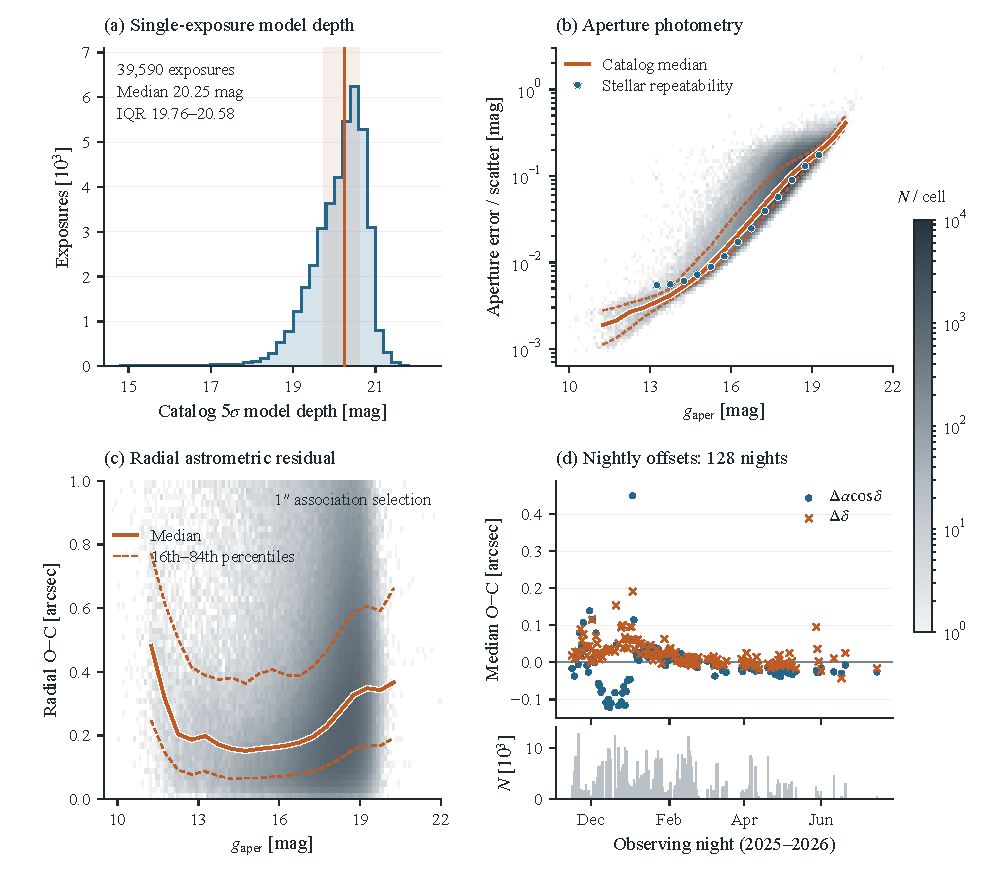
\includegraphics[width=\linewidth]{fig05_measurement_quality.pdf}
\caption{Measurement quality in the validated exposure sample.
(a) Catalog $5\sigma$ model depth for 39,590 exposures in 0.2-mag bins;
the orange line and shaded band mark the median and interquartile range.
(b) Reported aperture error for 500,092 unflagged primary associations
with positive magnitude error, flux, and flux error. Counts use
0.1-mag by 0.04-dex cells. In (b,c), solid and dashed orange curves show
the median and 16th--84th percentiles in 0.5-mag bins containing at least
30 measurements. Blue points in (b) show the stellar repeatability of
Equation~\ref{eq:repeatability} for the six selected field--night
sequences, using bins with at least 50 stellar pairs.
(c) Great-circle radial O$-$C separation, in 0.1-mag by $0.02\asec$
cells. The displayed magnitude range contains 531,416 of the 531,612
primary associations; 195 entries with placeholder magnitude 99 and
one entry at 23.18~mag fall outside it. The shared logarithmic color
bar gives counts per plotted cell. The astrometric distribution is
selected within $1\asec$.
(d) Nightly medians of the signed residuals for all 531,612
associations over 128 physical observing nights; the lower gray
bars give the number of associations in each night. The symbol
\gaper\ denotes the white-light scale defined in
Section~\ref{sec:facility}.}
\label{fig:quality}
\end{figure}

\subsection{Retention of already-detected known-object nights}
\label{sec:retention_results}

Applying the historical definition in
Section~\ref{sec:retention_method} gives 75,899 retained
object--nights out of 102,347 eligible detected
object--nights, or $R_{\rm cond}=74.16\%$. The formal
95\% Wilson interval is 73.89--74.43\%. This interval
summarizes binomial counting uncertainty for the specified
cohort; it does not include correlations among nights or
uncertainty in the sample selection.

Figure~\ref{fig:retention} resolves the result in median
object--night \gaper\ and predicted first-to-last angular rate.
The count map shows where the eligible sample constrains this test,
and the adjacent map gives the retained fraction in the same cells.
The one-dimensional panels summarize the marginal behavior with
their corresponding sample counts. The lowest-rate bin, $3$--$5$~\rateunit,
retains 566 of 1,400 object--nights (40.43\%). The
brightest bin, $10\leq\gaper<13$, retains 262 of 643
(40.75\%). The loss at these edges shows why a single
aggregate fraction does not fully describe the processing.
Source filtering, available displacements, sampling,
and the composition of each detected subset all enter
the result.

Reconstructing the eligible object--night sample from validated
exposures and physical observing nights gives 75,467 linked
object--nights out of 101,784 (74.14\%) over 126 nights.
This calculation reuses the original pre-subtraction links and
retains the historical processing-state policy. Restricting the same
selection to nonquarantined nights with readable stage products gives
73,787/99,426 (74.21\%) over 122 nights. The close agreement with
74.16\% shows that the aggregate result changes little after
exposure and time reconciliation; the three sample definitions are
preserved separately in the accompanying tables.

\begin{figure}[tbp]
\centering
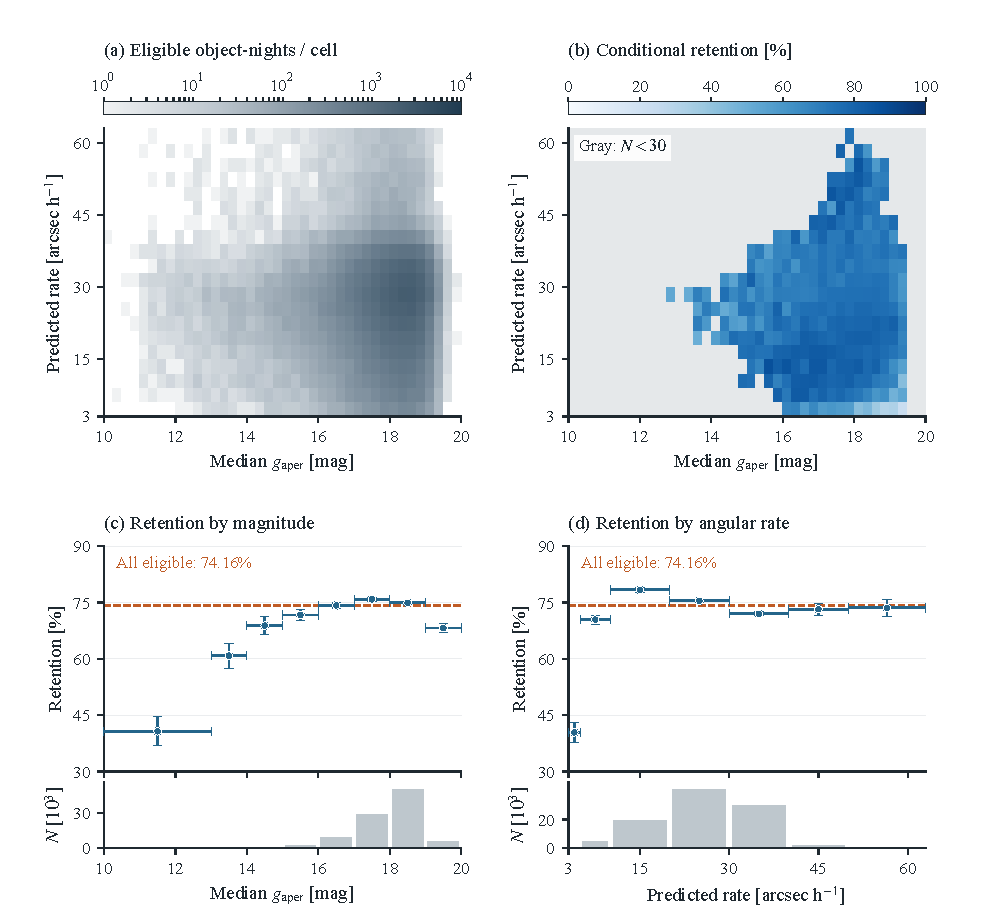
\includegraphics[width=\linewidth]{fig06_conditional_retention.pdf}
\caption{Conditional linkage retention in the historical object--night
sample. Eligibility requires at least three detections associated
with one identity within $1.5\asec$ and a predicted first-to-last
rate of $3$--$63$~\rateunit. A retained object--night is represented
by an existing link with at least three members mapping to that
identity. (a) Eligible counts in 0.25-mag by
3~\rateunit\ cells, on a logarithmic color scale.
(b) Retained fractions in the same cells; cells with fewer than
30 eligible object--nights are masked in gray.
(c,d) One-dimensional retained fractions with 95\% Wilson intervals
and horizontal bars spanning the bins. The lower histograms show
eligible counts per bin. The dashed line is the full historical
fraction, 75,899/102,347 (74.16\%).
The magnitude-dependent panels (a--c) contain 102,315 eligible
object--nights and 75,897 retained cases. They omit 32 object--nights
with unusable magnitudes, including two retained cases, which remain
in the overall and rate-dependent samples. Both two-dimensional
maps use unsmoothed counts. These panels retain the original
processing cohort; the exposure-validated comparison is given in
the text.}
\label{fig:retention}
\end{figure}
